\documentclass{article}
\usepackage{graphicx} % Required for inserting images
\usepackage[a4paper,margin=2.5cm]{geometry}
\usepackage{amsmath}
\usepackage{float}
\usepackage{xcolor}
\usepackage{listings}
\usepackage{caption}
\usepackage{subcaption}
\usepackage{xparse}
\usepackage{hyperref}
\usepackage{amssymb}
\usepackage{verbatim}
\usepackage{fancyhdr}
\pagestyle{fancy}
\usepackage{xspace}
\cfoot{}
\lfoot{SMOS, Universitat Politècnica de Catalunya, year 2023-24}
\rfoot{\thepage}

\definecolor{codegreen}{rgb}{0,0.6,0}
\definecolor{codegray}{rgb}{0.5,0.5,0.5}
\definecolor{codepurple}{rgb}{0.58,0,0.82}
\definecolor{backcolour}{rgb}{0.95,0.95,0.92}

\lstdefinestyle{mystyle}{
    backgroundcolor=\color{backcolour},   
    commentstyle=\color{codegreen},
    keywordstyle=\color{magenta},
    numberstyle=\tiny\color{codegray},
    stringstyle=\color{codepurple},
    basicstyle=\ttfamily\footnotesize,
    breakatwhitespace=false,         
    breaklines=true,                 
    captionpos=b,                    
    keepspaces=true,                 
    numbers=left,                    
    numbersep=5pt,                  
    showspaces=false,                
    showstringspaces=false,
    showtabs=false,                  
    tabsize=2
}

\lstset{style=mystyle}

\title{\textbf{Random Walk}}
\author{Student: Giacomo Calabria}
\date{}

\begin{document}

\maketitle

\section*{Introduction}
In this second module we use random walk method in order to find electrostatic potential distribution inside of a square box or in a space with more complicated geometry. The problem under consideration is finding solution to Laplace equation in two dimension in an area bounded by a square box.\\
Given the value of the electrostatic potential at all points at the boundary, which are at the edges of the box and any shape inside of the box. The electrostatic potential at all interior points satisfy the Laplace equation
\begin{equation}
    \frac{\partial^2\phi}{\partial^2x}+\frac{\partial^2\varphi}{\partial^2y}=0
\end{equation}
Its possible to reformulate the problem of finding an electrostatic potential in a box with specified values of the potential at the edges as a random walk problem.
\subsection*{Discrete Random Walk algorithm}
The algorithm of Discrete Random Walk begins by selecting a point $(xy)$ where the potential value requires estimation. Proceed by taking random steps along the $x$ and $y$ directions until reaching the boundary, collecting potential values at these boundary points $V_b(i)$. This process repeats $M$ times, with the potential at the boundary accumulating after each iteration.\\\\To estimate the potential $V(xy)$ at point $(xy)$, the total sum of potential values at the boundary is divided by the number of random walkers.
\begin{equation}
    V(x,y)\approx\frac1M\sum_{i=1}^M{V_b(i)}
\end{equation}
\section{Electrostatic potential in a square box}
Considering a square box with unitary side. Where the left side has potential +10 and the others have potential equal to +1. The whole square is divided into a mesh containing $N\times N$ equally spaced lattice sites. After implementing a discrete random walk algorithm for solving the Laplace equation we report the dependence of the obtained potential on $(x,y)$ with an heatmap.\\\\
Using the following code to perform a random walk
\begin{lstlisting}[language=Python]
def random_walk(x, y):
    while True:
        x += random.choice([-1, 0, 1])  # Choose a random move and update the position
        y += random.choice([-1, 0, 1])
        # Check if we reach an boundary
        if y <= 0:
            return 10
        if y >= N:
            return 1
        if x <= 0:
            return 1
        if x >= N:
            return 1
\end{lstlisting}
\clearpage \noindent And with the following code we perform the random walks for each position in the box
\begin{lstlisting}[language=Python]
N = 100 # number of sites in the box
M = 120 # number of random walk per position

Box1 = np.zeros((N,N))
for i in range(N):
    for j in range(N):
        temp = sum(random_walk(i, j) for _ in range(M))
        Box1[i][j] = temp/M #Compute the estimated potential
        
plt.imshow(Box1, cmap='gnuplot', interpolation='bilinear')
\end{lstlisting}
We report the generated heatmap of the electrostatic potential field in \autoref{fig:1}
\begin{figure}[H]
    \centering
    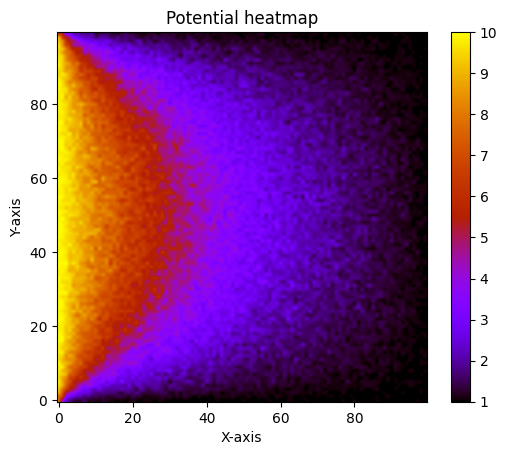
\includegraphics[width=.7\linewidth]{images/Figure1.png}
    \caption{}
    \label{fig:1}
\end{figure}
\clearpage
\section{Electrostatic potential of a plane condenser}
We now consider a two-dimensional model for a plane condenser composed of two finite-width plates of opposite potential. The voltage corresponds to the difference of the potentials on the plates while zero potential can be imposed at the edges of the box. We use Gaussian displacement in a continuous space to generate a sufficiently large number of Random Walks and estimate the potential value according to the average over the boundary values.\\\\
We modified the function that performs the random walk, considering now that there is a plane condenser inside the box.
\begin{lstlisting}[language=Python]
C1 = N/3 # position of the first plate of the condenser
C2 = 2*N/3 # position of the second plate of the condenser
def random_walk(x, y):
    while True:
        x += random.choice([-1, 0, 1])  # Choose a random move and update the position
        y += random.choice([-1, 0, 1])

        if x >= N:  # Check if it is arrived at one plate or outside the box
            return 0
        if y >= N:
            return 0
        if y <= 0:
            return 0
        if x <= 0:
            return 0
        if (y >= C1-2 and y <= C1+2) and (x >= 3/10*N and x <= 7/10*N):
            return 1
        if (y >= C2-2 and y <= C2+2) and (x >= 3/10*N and x <= 7/10*N):
            return -1
\end{lstlisting}
The code that perform the random walks for each position is the same. We report the generated heatmap of the electrostatic potential field in \autoref{fig:2}
\begin{figure}[H]
    \centering
    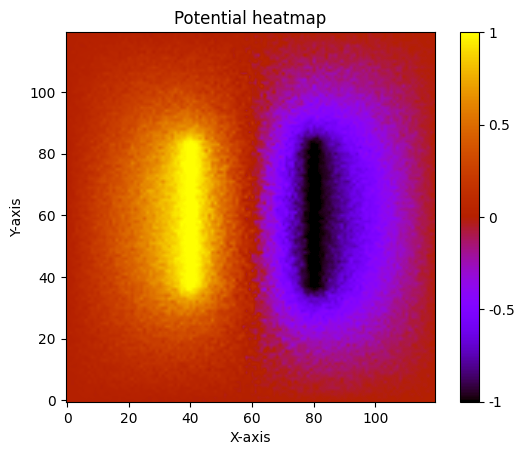
\includegraphics[width=.7\linewidth]{images/Figure2.png}
    \caption{}
    \label{fig:2}
\end{figure}
\clearpage
\subsection{Electric field}
We wanna now estimate the amplitude of the electric filed $E(x,y)$ its vector value corresponds to the anti gradient of the potential field, $\Vec{E}=-\nabla V$, but the amplitude can be approximated as 
\begin{equation}
    E(x,y)\approx\sqrt{\left[\frac{V(x+\Delta x,y)-V(x,y)}{\Delta x}\right]^2+\left[\frac{V(x,y+\Delta y)-V(x,y)}{\Delta y}\right]^2}
\end{equation}
\noindent Using the following code we compute the electric field from the potential using finite differences.
\begin{lstlisting}[language=Python]
for i in range(1, N-1):
    for j in range(1, N-1):
        Ex = (Box2[i+1][j] - Box2[i-1][j])/2
        Ey = (Box2[i][j+1] - Box2[i][j-1])/2
        Box3[i][j] = np.sqrt(Ex**2 + Ey**2)

# Plot the Box into an image as heatmap
plt.imshow(Box3, cmap='gnuplot', interpolation='bilinear')
\end{lstlisting}
We report the generated heatmap of the electric field in \autoref{fig:3}
\begin{figure}[H]
    \centering
    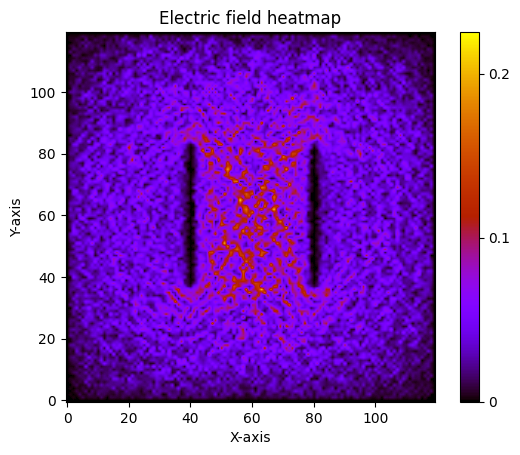
\includegraphics[width=.7\linewidth]{images/Figure3.png}
    \caption{}
    \label{fig:3}
\end{figure}
\noindent We can see that the effects of the statistical noise is amplified in the calculation of the electric field, as difference of the potential is calculated.
\end{document}